In this section we briefly summarise the results of the ML analysis performed
on the data.
We will explore several diverse algorithms including regularised versions of
the linear regression (LR, from now on), support vector machines (SVM),
decision trees (random forests, RF, and gradient boosted decision trees, GBDT),
and artificial neural networks (ANN).
For each algorithm we fit the data on training set and evaluate it on the
validation set to perform the optimisation of the \textit{hyperparameters}
using Bayes statistics.
The goal is to minimise the objective function, that is the validation MSE,
without knowing its analytic form, by only inferring the probability of
obtaining a better result with a different choice of hyperparameters.

\subsection{Regression Analysis}\label{sec:ml:regr}

In \Cref{tab:ml:test} we summarise the results obtained from prediction on the
test set for the algorithms used: in particular the first four lines refer to
linear models (LR is the plain regression, EN implements both $l_1$ and $l_2$
regularisation, Lasso and Ridge separately implement $l_1$ and $l_2$
regularisation, respectively); l-SVR is the linear implementation of the SVM
models, while r-SVR uses a Gaussian \textit{kernel trick}; RF and GBDT are
different ensemble algorithms based on decision trees (namely random forests
and gradient boosted trees); ANN represents the neural network architecture (no
hidden layers, only one input layer with 30 units, batch normalisation layer
and a dropout layer with 0.1 drop rate leading to a network of 691 trainable parameters and 60 fixed parameters).

\begin{table}[htbp]
\centering
\resizebox{0.475\textwidth}{!}{%
\begin{tabular}{@{}lcccc@{}}
\toprule
         &             MSE &              MSE 95\% CI &  MAE &                   R2 \\
\midrule
LR       &            0.13 &           $[0.07, 0.20]$ & 0.27 &                 0.74 \\
EN       &            0.19 &           $[0.12, 0.27]$ & 0.33 &                 0.62 \\
Lasso    &            0.20 &           $[0.13, 0.28]$ & 0.34 &                 0.60 \\
Ridge    &            0.13 &           $[0.07, 0.20]$ & 0.27 &                 0.74 \\
l-SVR    & $8 \times 10^3$ & $[-3, 20] \times 10^{3}$ &   20 & $-1.6 \times 10^{4}$ \\
r-SVR    &           0.030 &                      --- & 0.08 &                 0.95 \\
RF       &           0.013 &                      --- & 0.05 &                 0.97 \\
GBDT     &          0.0010 &                      --- & 0.02 &                 1.00 \\
ANN      &           0.006 &                      --- & 0.05 &                 0.99 \\
\bottomrule
\end{tabular}
}
\caption{Summary of the predictions on the test set for the different
algorithms. We present the MSE, the Mean Absolute Error (MAE) and the
$R^2$ score. The confidence intervals of the MSE are present only for linear
models since they rely on statistical assumptions on the distribution of the
residuals (they are normally distributed).}
\label{tab:ml:test}
\end{table}

\begin{figure}[htbp]
  \centering
  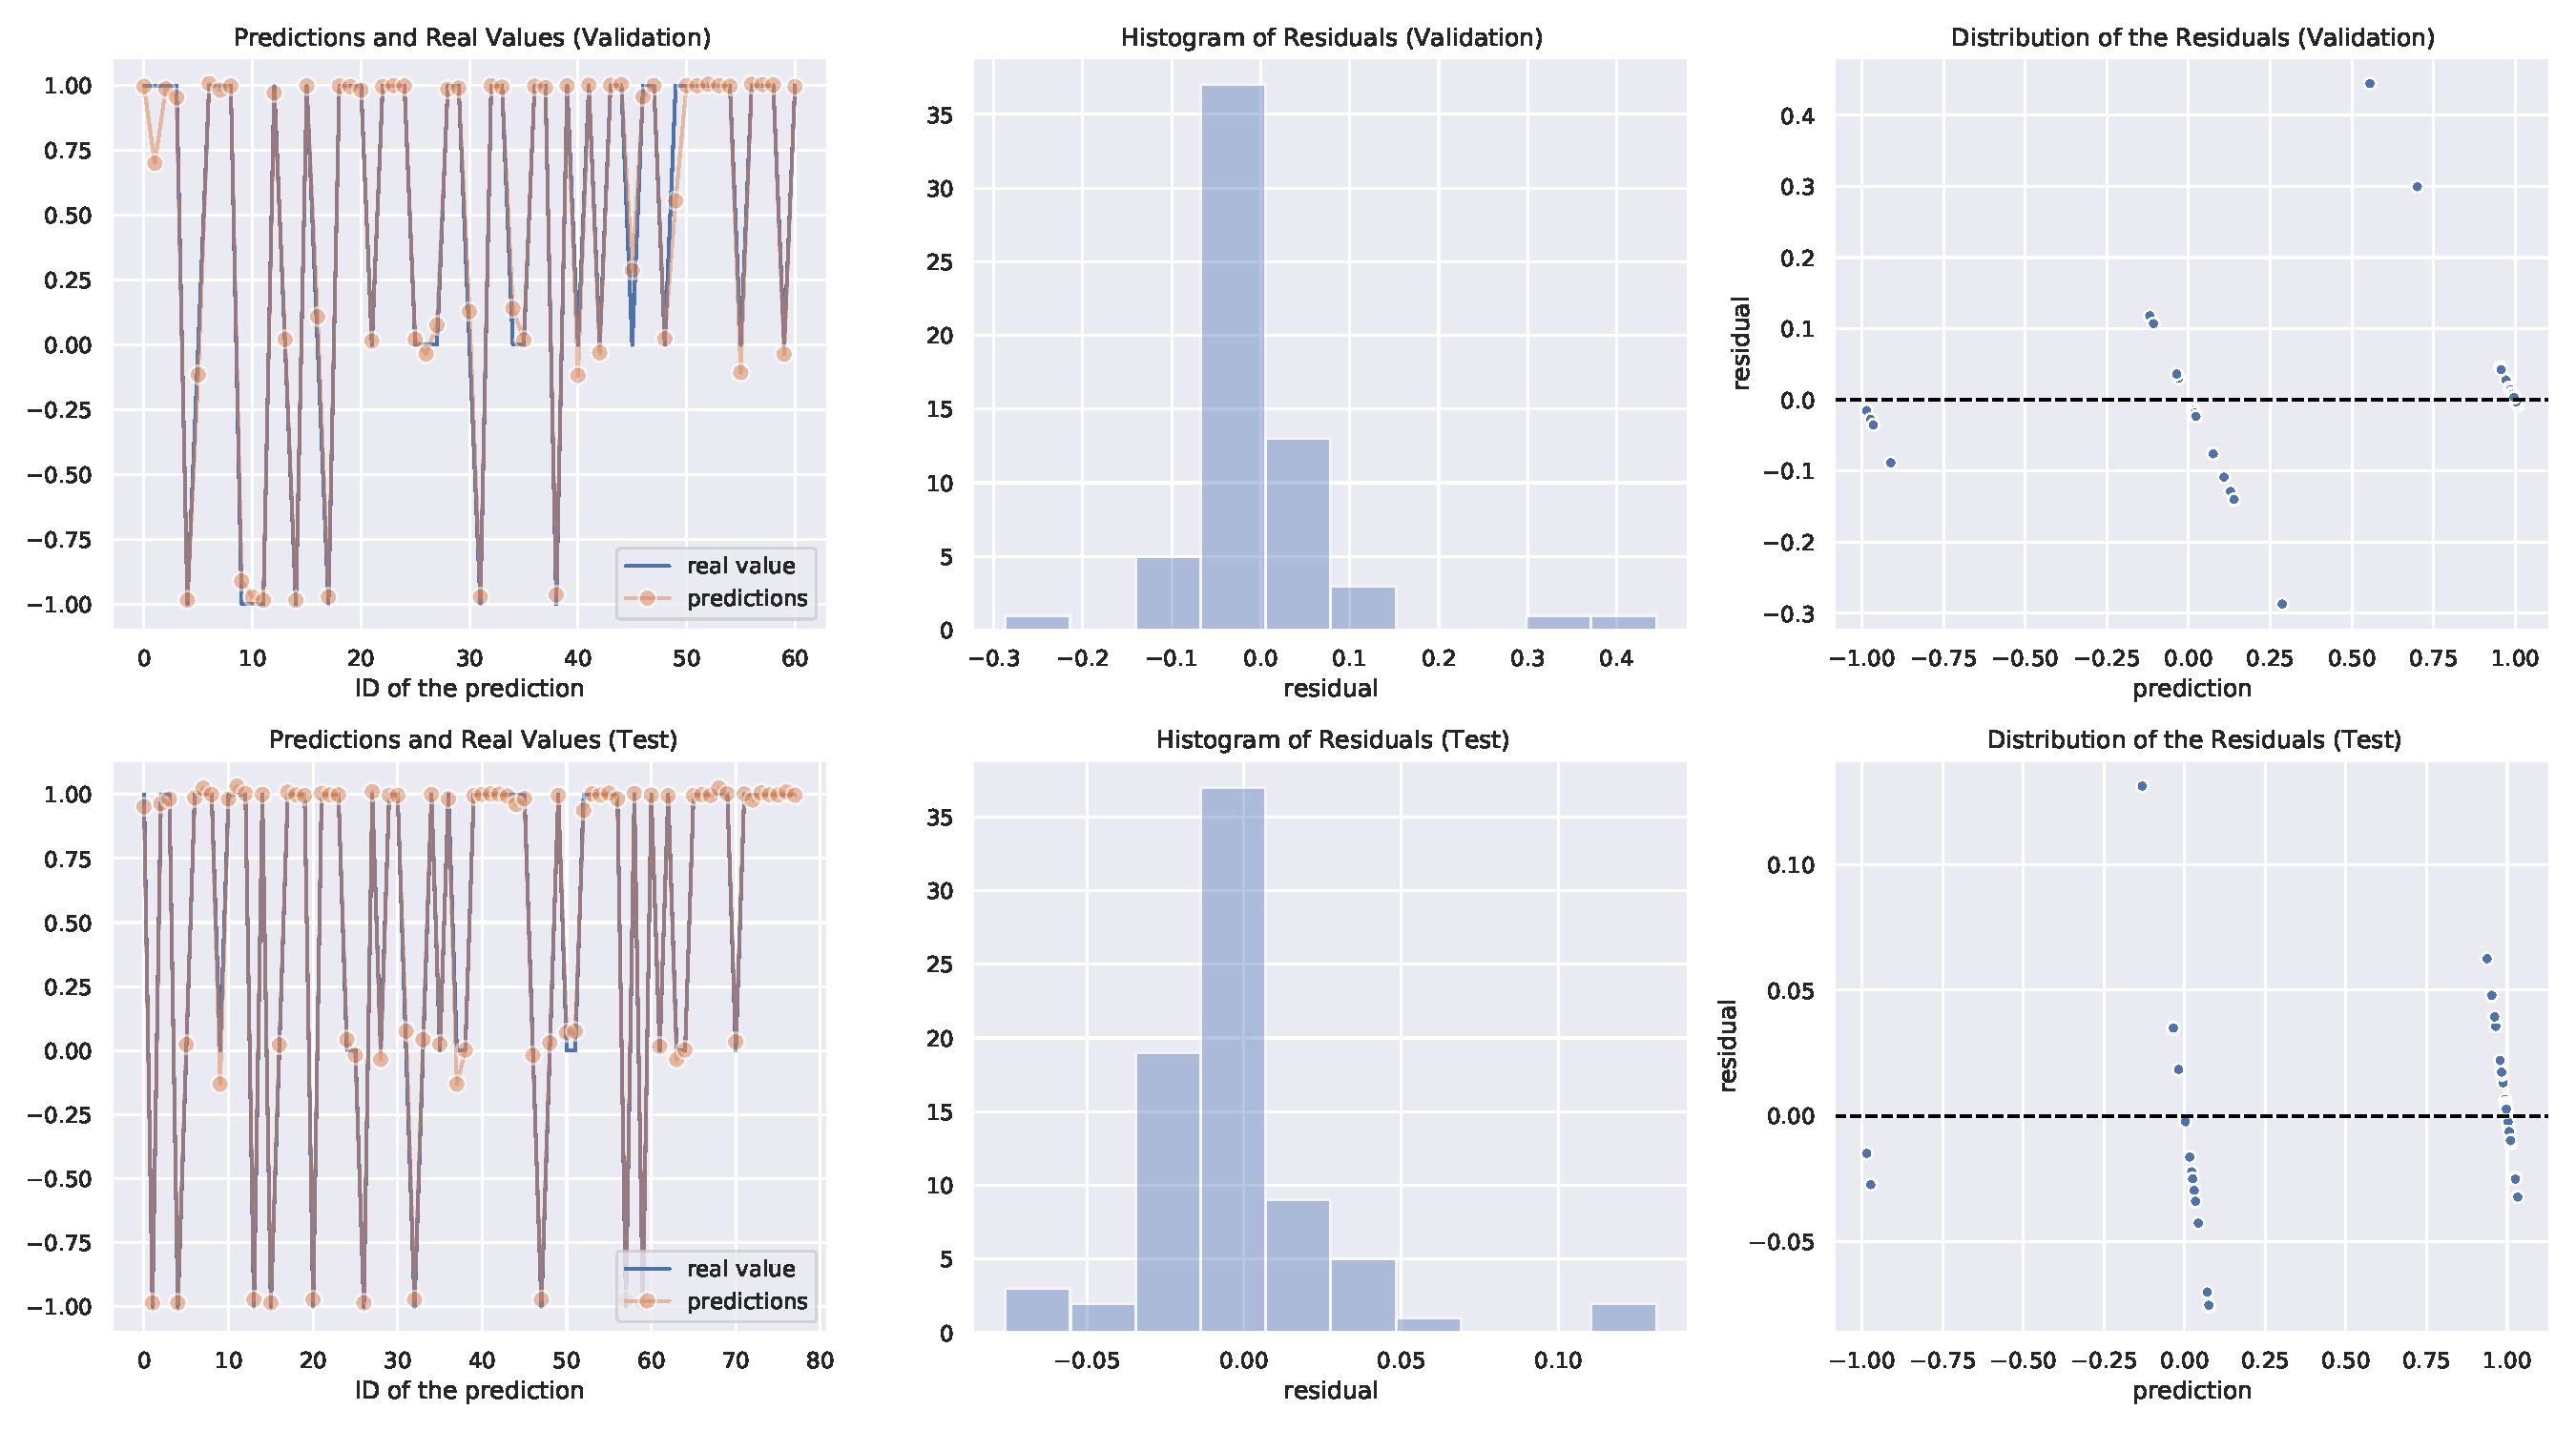
\includegraphics[width=0.475\textwidth]{img/grd_bst}
  \caption{GBDT validation and test sets residuals.}
  \label{fig:ml:gbdt}
\end{figure}

As we can see the GBDT are able to deliver the best results both in
terms of MSE and R2 score followed by the implementation of the shallow
network (trained over 5000 epochs: training is fairly rapid but trees are by
far faster).
On the other hand $l_1$ regularisation (both alone and in combination with
$l_2$) fails to approximate well the prediction labels. In the same fashion the
l-SVR fails completely.

In \Cref{fig:ml:gbdt} we show the validation and test set distribution of the
predictions and residuals.
As we can see the algorithm correctly approximates the \texttt{exp} labels with
residual contained in a small interval.
There is however a general tendency to underestimate the \texttt{exp} $= -1$
label and to overestimate \texttt{exp} $= 1$: in linear model this would have
signalled an incomplete model since residuals seem to be correlated with
predictions, but in the case of decision trees it does not pose an issue.

\begin{figure}[htbp]
  \centering
  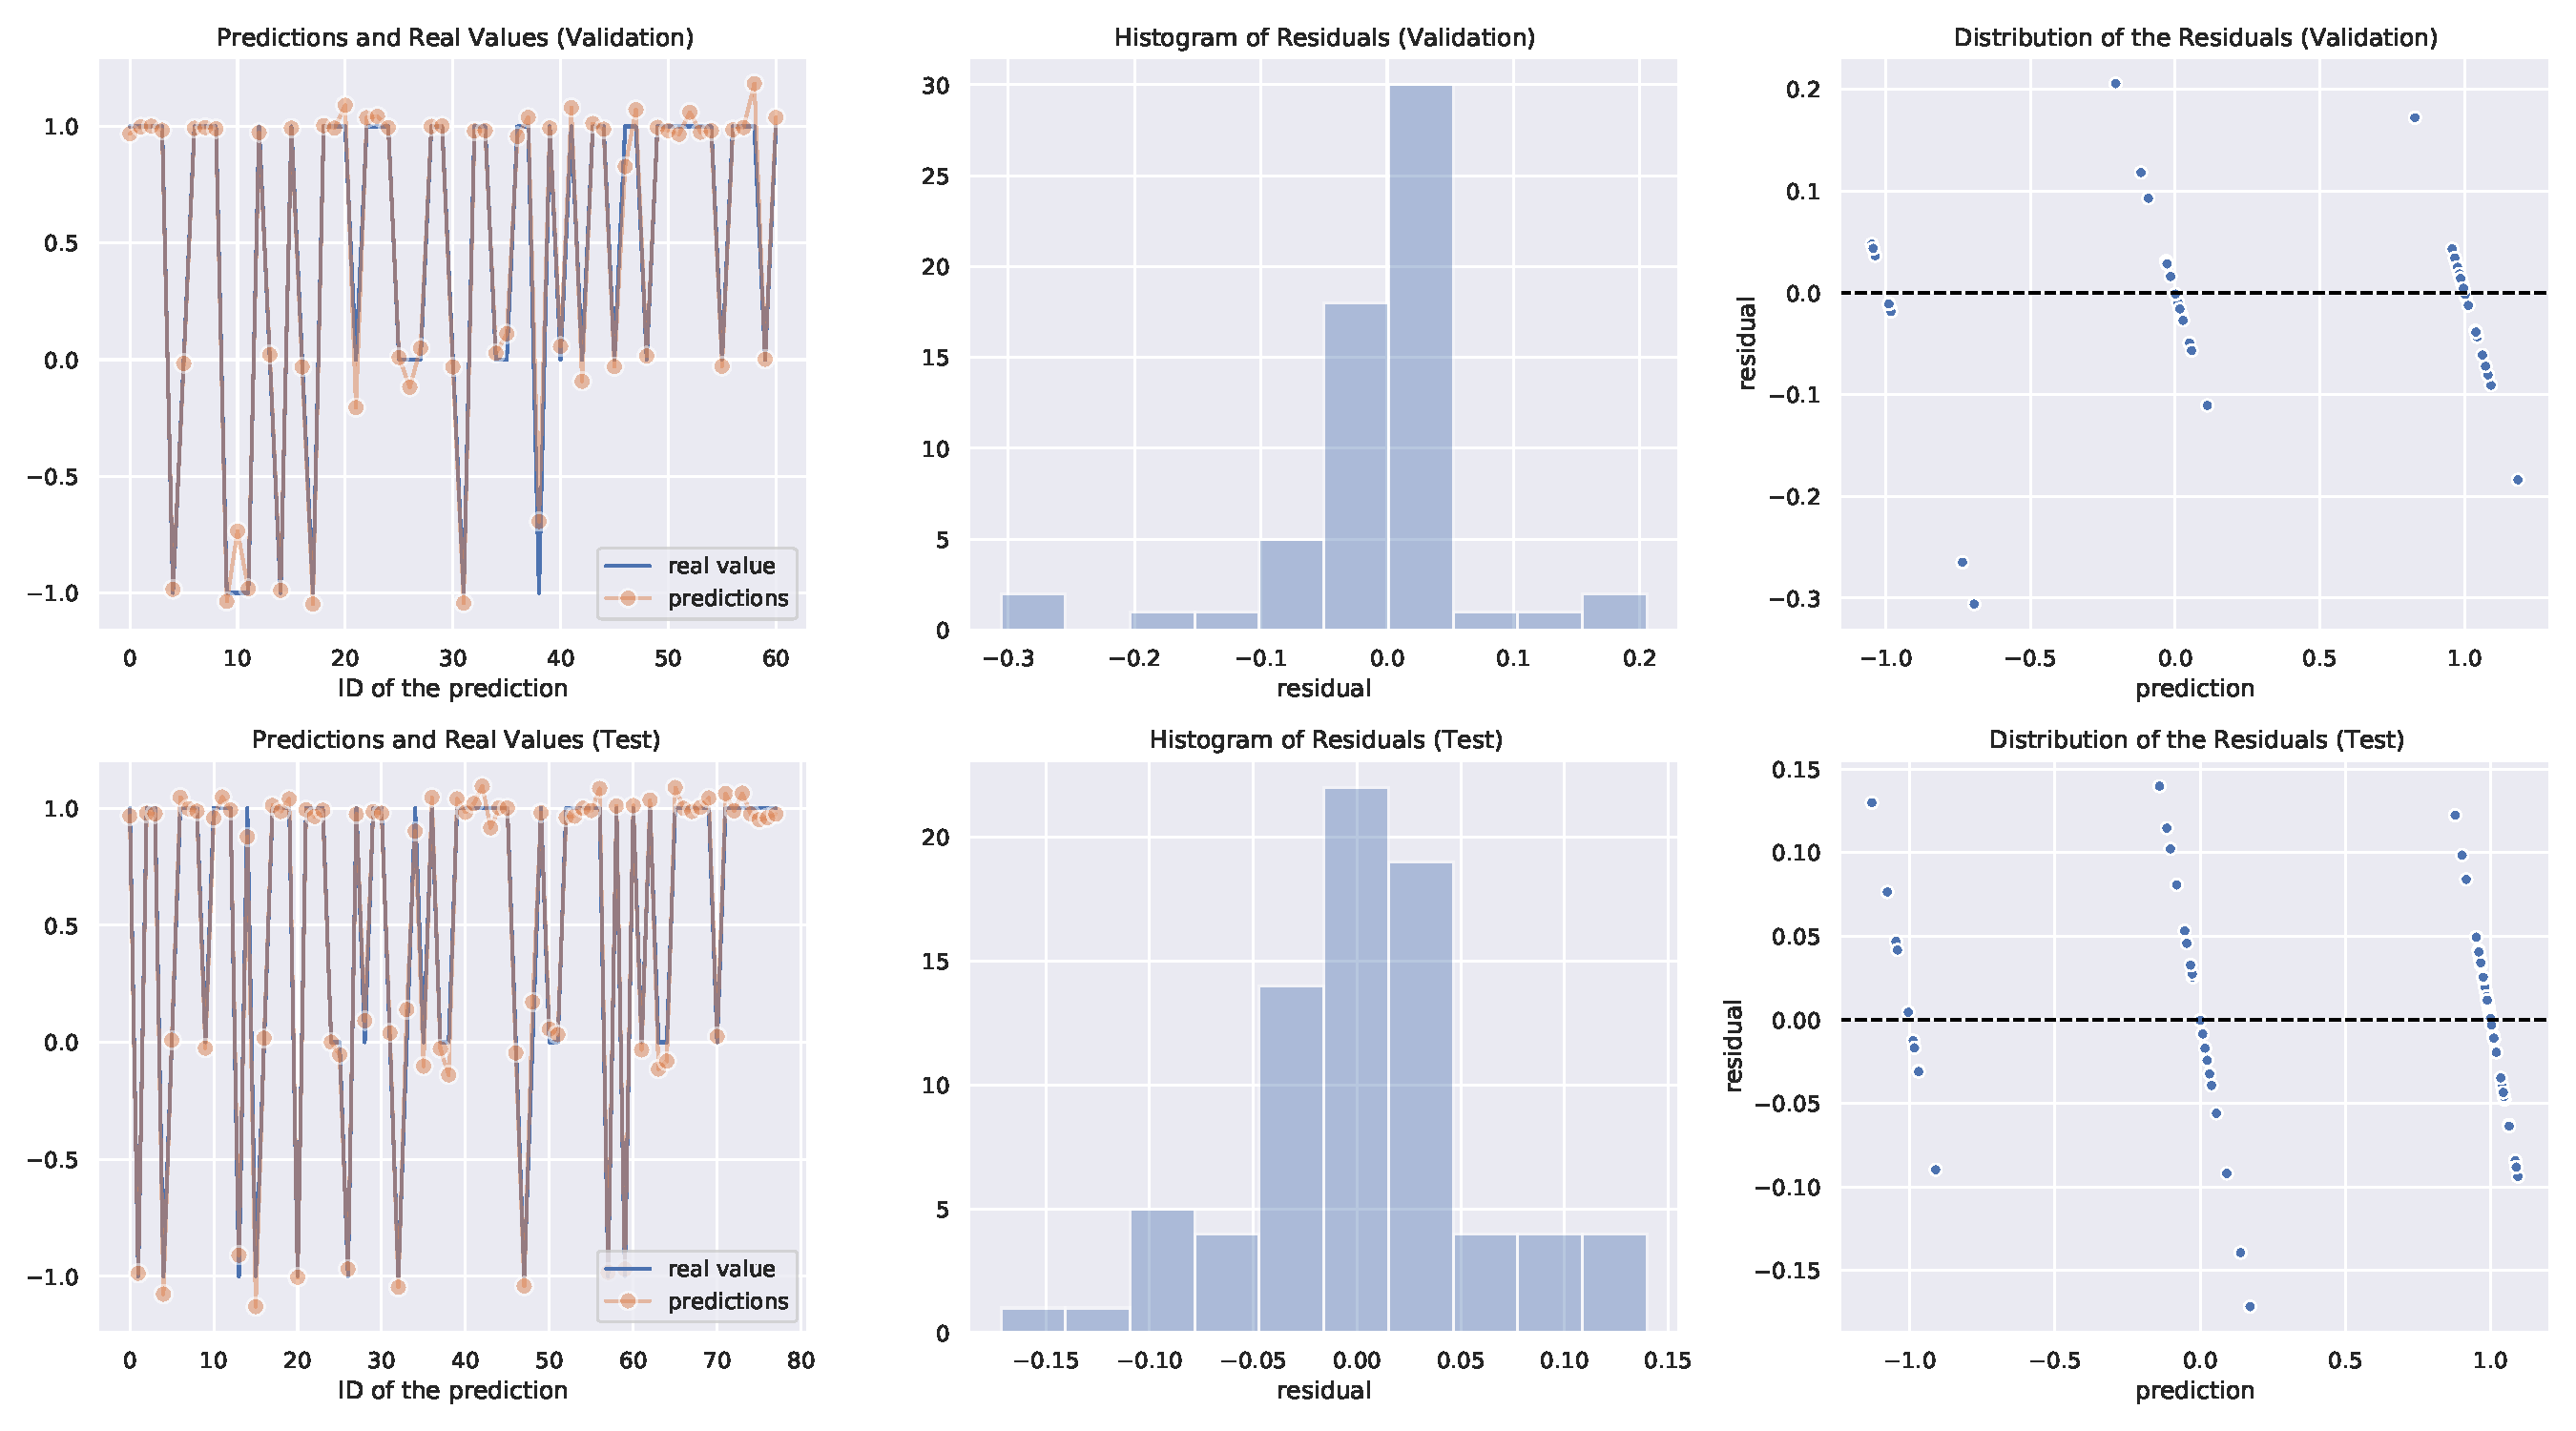
\includegraphics[width=0.475\textwidth]{img/ann_mod}
  \caption{ANN validation and test sets residuals.}
  \label{fig:ml:ann}
\end{figure}

In \Cref{fig:ml:ann} we show the same plot generated from the ANN predictions.
As for the GBDT, the ANN is correctly trying to predict the \texttt{label} with
very small residuals.
Differently from the GBDT, residuals are more randomly distributed for each
prediction and no pattern is recognisable.

\begin{table}[htbp]
\centering
\begin{tabular}{@{}lcc@{}}
\toprule
                  & \textbf{RF} & \textbf{GBDT} \\
\midrule
no.\ leaves       & 48          & 15            \\
max depth         & 300         & 17            \\
no.\ estimators   & 25          & 3439          \\
subsample         & 0.85        & 0.99          \\
colsample by tree & 0.7         & 1.0           \\
min child weight  & 0.01        & 0.1           \\
$l_1$ reg.        & 0.16        & 1.0           \\
$l_2$ reg.        & 0.20        & $10^3$        \\
learning rate     & ---         & 0.1           \\
\bottomrule
\end{tabular}%
\caption{Hyperparameters choices for RF and GBDT.}
\label{tab:ml:hyper}
\end{table}

In \Cref{tab:ml:hyper} we show a summary of the hyperparameters used for
training RF and GBDT: as expected the optimisation process chose a small number
of fully grown trees in the first case, while it led to a large number of
boosting rounds of shallow trees in the latter.

\subsection{Feature Explanation}\label{sec:ml:shap}

As a last step in the analysis, we use the trained trees (for simplicity) and
study their properties to possibly show how each training feature plays inside
the algorithm and how the final prediction is determined.
For this analysis we will study the Shapley values computed as the difference
between each permutation of subsamples of the features and compare the results
with the average of the final prediction in order to see which variable is
pushing the results and which variable is dragging it.
We will also consider the variable ranking provided naturally by the decision trees to determine which feature plays a larger role for the final prediction.

\begin{figure}[htbp]
  \centering
  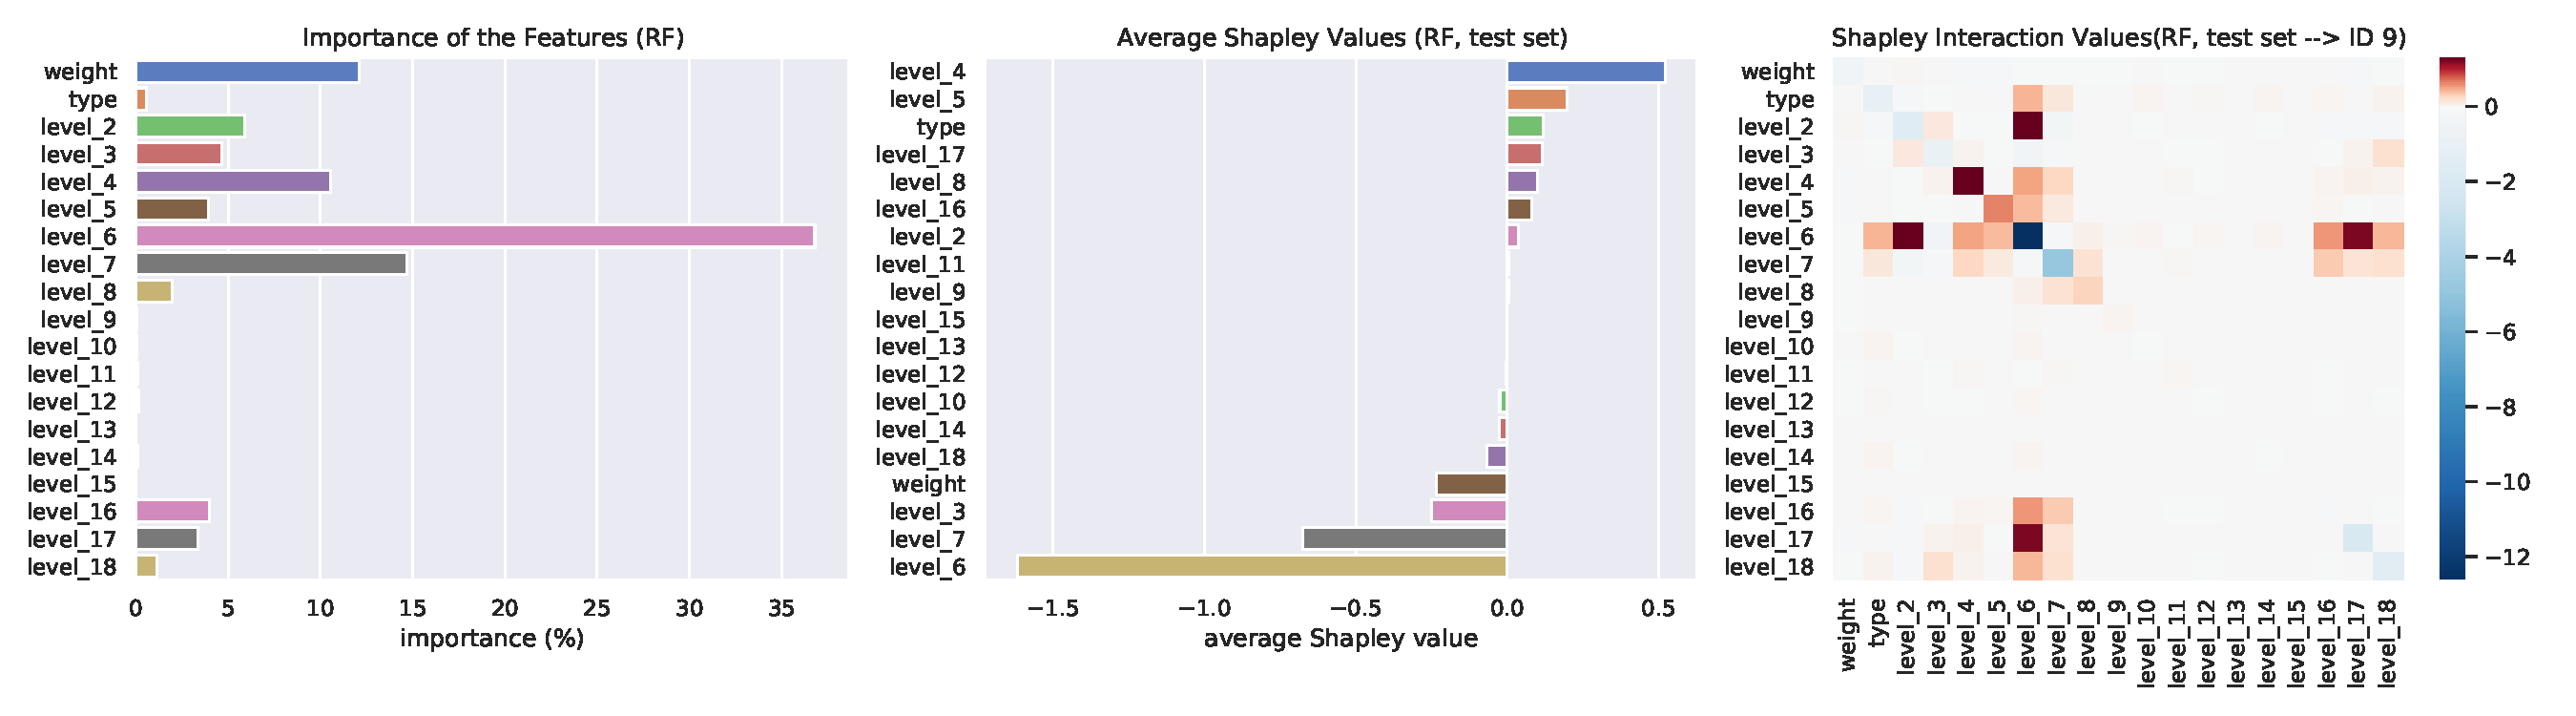
\includegraphics[width=0.475\textwidth]{img/rnd_for_shapley}
  \caption{Variable ranking and Shapley values (computed on the test set) of
  RF.}
  \label{fig:ml:rnd_for_shap}
\end{figure}

In \Cref{fig:ml:rnd_for_shap} we show the variable ranking and the Shapley
values for the RF algorithm.
The first plot shows that RF rely mostly on low and high truncation orders in
the top levels of the trees to better discriminate the predictions, even though
\texttt{weight} is still the most important feature (as we could have expected
from the results of the EDA).
The average Shapley values (second plot) show that most features give a comparable contribution to the prediction, exception made for one of them which seems to drive the final result in a more direct way.
Finally the \textit{interacting Shapley values} (taken for a random sample in
the test set) in the third plot show that the whole set of variables is mostly
non interacting except very sporadic contributions between distant levels.

\begin{figure}[htbp]
  \centering
  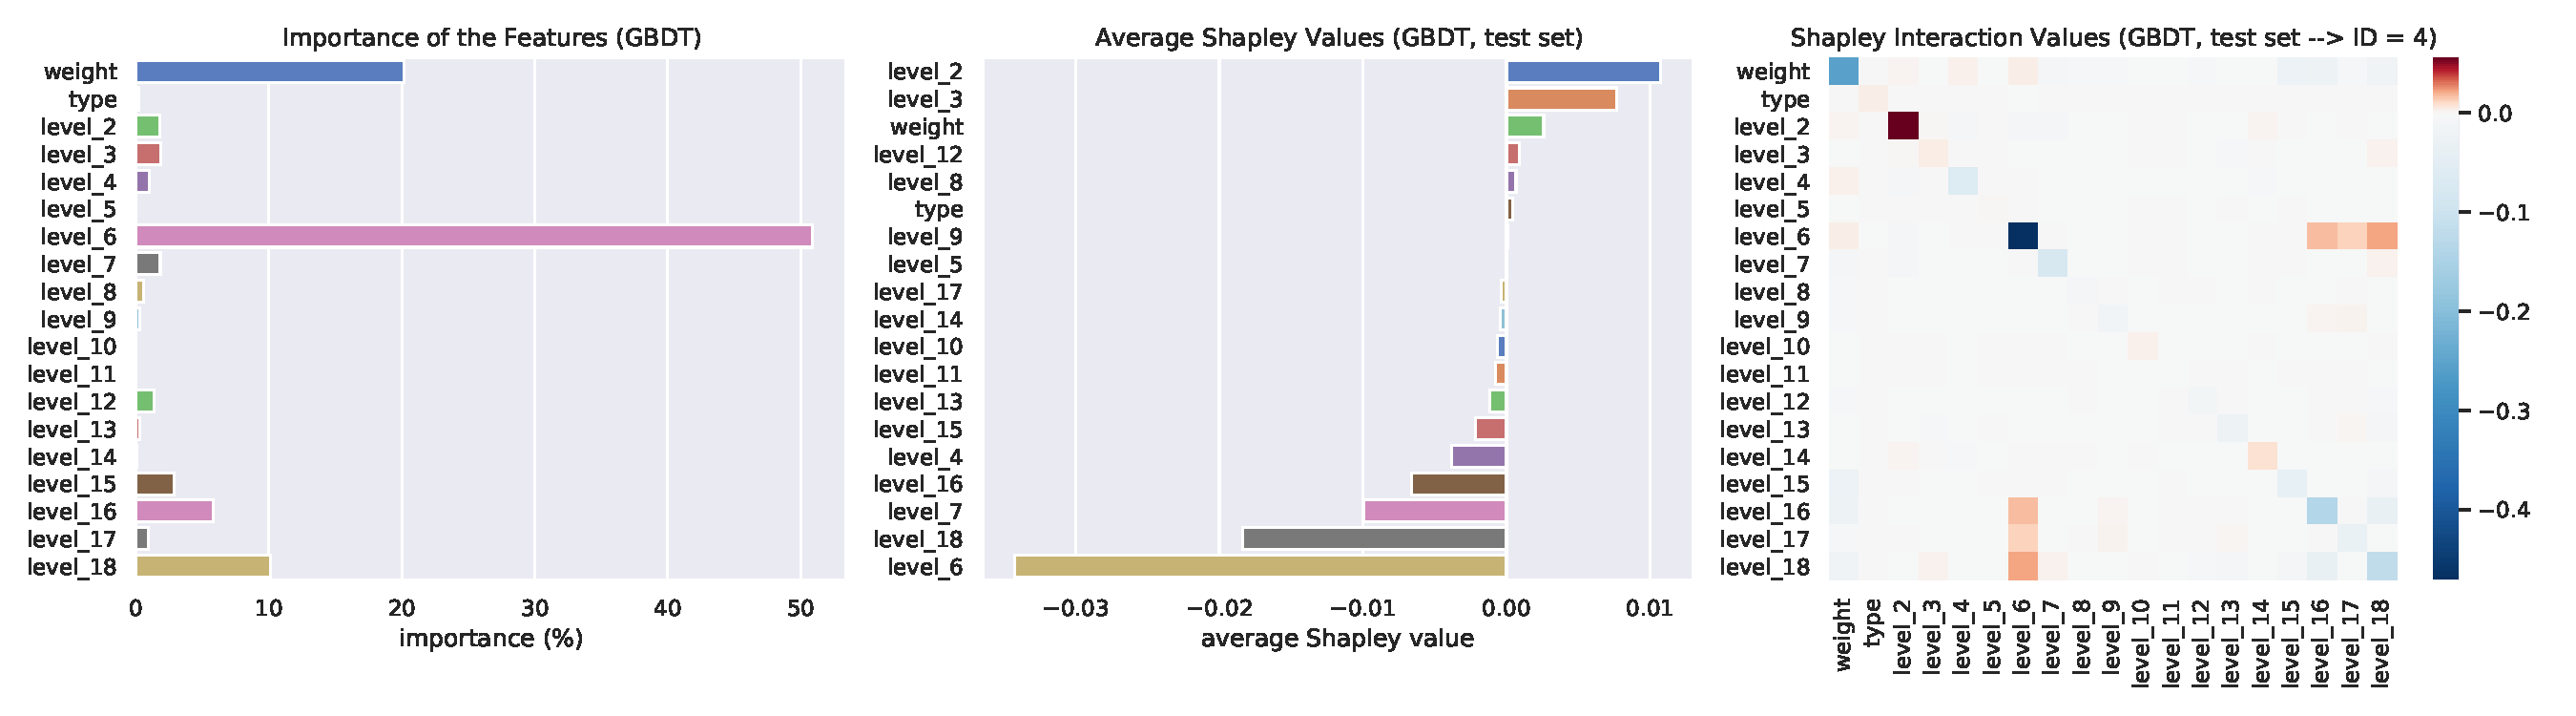
\includegraphics[width=0.475\textwidth]{img/grd_bst_shapley}
  \caption{Variable ranking and Shapley values (computed on the test set) of GBDT.}
  \label{fig:ml:grd_bst_shap}
\end{figure}

In \Cref{fig:ml:grd_bst_shap} we finally show the same plot for the GBDT.
Differently from the RF, GBDT seem to attach greater importance also to the
central truncation levels while disregarding almost completely the categorical
variable (for this particular algorithm it could have been removed but the
corresponding Shapley value shows that its relevance is so marginal that the
result would not have changed).
